% =====================================================================
%  Experiment 15 — Attack-token -> query information flow in monoT5
%  Compile with:  pdflatex 15_monot5_attack_to_query_flow_report.tex (twice)
%  Figure paths are relative to this file (outputs/plots/...), so compile
%  from the 15_monot5_attack_to_query_flow/ directory.
% =====================================================================
\documentclass[11pt]{article}

\usepackage[margin=1in]{geometry}
\usepackage{amsmath, amssymb}
\usepackage{graphicx}
\usepackage{booktabs}
\usepackage{array}
\usepackage{float}
\usepackage{xcolor}
\usepackage{caption}
\usepackage{enumitem}
\usepackage[hidelinks]{hyperref}

\newcommand{\fwd}{\ensuremath{e^{\mathrm{fwd}}}}
\newcommand{\rev}{\ensuremath{e^{\mathrm{rev}}}}
\newcommand{\comb}{\ensuremath{e^{\mathrm{comb}}}}

\title{\textbf{Attack-Token $\rightarrow$ Query Information Flow in the monoT5 Encoder} \\[6pt]
\large Source-Specific Edge-Message Patching at the 18 Important Encoder Heads}
\author{Information-Retrieval Adversarial-Evaluation Project --- Experiment 15}
\date{September 2026}

\begin{document}
\maketitle

\begin{abstract}
Earlier experiments showed that keyword-stuffing attacks on
\texttt{castorini/monot5-base-msmarco} change the \emph{query}-token
representations even though the injected tokens sit in the document, and that
18 encoder self-attention heads carry the attack effect. Neither result shows
\emph{how} attack information reaches the query. We intervene directly on the
source-specific attention message
$m(q)=\sum_{a\in A}P[q,a]\,V[a]$ from the injected positions $A$ to the query
positions $q$, head by head, before the output projection. We swap it
between the attacked run and a length-matched padded control in both the
sufficiency (forward) and necessity (reverse) directions, across all 105
attacks (5{,}250 successful examples).

Six of the 18 heads pass the pre-registered one-sided sign-flip test after
Benjamini--Hochberg correction: L8H11, L10H2, L11H4, L10H4, L10H6 and L10H0.
Their forward and reverse recoveries agree closely, so the direct
attack$\rightarrow$query edge is both sufficient and necessary for a
\emph{part} of the attack. That part is small. Using a pooled
ratio-of-means, the strongest head (L8H11) explains $\approx 8.5\%$ of the
attack effect and the others 1--4\%, while their whole-head effects are
several times larger. The one exception is L8H11, whose edge effect exceeds
its whole-head effect. Two heads (L11H5, L9H3) carry an attack$\rightarrow$query
message that works \emph{against} the attack. The equal-weight mean of
per-example ratios (the pre-registered headline) is strongly inflated by
examples with near-zero attack effect, and we report robust descriptive
summaries alongside it.
\end{abstract}

\section{Question and motivation}
Experiments 1 and 6 localised the attack effect to late encoder self-attention
(layers 10--11) and showed that patching \emph{query} positions recovers part
of it. Experiment 11 found the effect sparse over encoder heads and flagged
18 of 144 heads (combined effect $>0.02$). Experiment 12 localised it within
query tokens, and Experiment 13 traced encoder$\rightarrow$decoder paths. Two
gaps remained:
\begin{itemize}[nosep]
\item Query-position patching shows \emph{that} query states carry attack
  information, not \emph{by which route}: a direct attack$\rightarrow$query
  attention message, a multi-hop relay through document or template
  positions, or earlier-layer effects.
\item Whole-head patching replaces a head's output at every position and for
  every source, so it cannot isolate one route. Attention weights are not
  enough either: Exp.~11 found that most important layer-10/11 heads have
  unremarkable attention mass.
\end{itemize}
\textbf{Question.} Do the 18 important heads make the attack work partly by
\emph{directly} moving information from the injected positions to the query
positions?

\section{Method}
\subsection{Edge message}
For encoder layer $L$, head $h$ (with $d_{kv}=64$) and target position $q$,
let $P[q,j]$ be the post-softmax attention and $V[j]$ the per-head value.
Then
\[
z(q)=\sum_j P[q,j]V[j],\qquad m(q)=\sum_{a\in A}P[q,a]V[a],
\]
where $z(q)$ is head $h$'s slice of the \texttt{.o} input and $A$ is the set
of \emph{all} injected token positions of the example (every repetition and
every scattered span), taken from Exp.~01's token alignment. The targets are
the exact SentencePiece positions of the query text (Exp.~06 spans), with
template tokens excluded. The hook points were verified against the
installed \texttt{transformers}~5.9 \texttt{T5Attention}, and
$z=\sum_j PV$ holds on every example (max error $2.9\times10^{-5}$).

\subsection{Interventions}
The padded control (Type B) has the attacked input's length, with pads
(attention mask 0) at $A$. Its message $m_{\text{ctrl}}$ is computed
explicitly, and was exactly $0$ on all 5{,}250 examples.
\begin{itemize}[nosep]
\item \textbf{Forward (sufficiency).} Receiver = control:
  $z\leftarrow z_{\text{ctrl}}-m_{\text{ctrl}}+m_{\text{atk}}$.
\item \textbf{Reverse (necessity).} Receiver = attack:
  $z\leftarrow z_{\text{atk}}-m_{\text{atk}}+m_{\text{ctrl}}$.
\end{itemize}
Only head $h$'s slice at the target positions changes. Other heads,
positions and source contributions are untouched, with no attention
renormalization. The model then runs forward normally, and the score is
$\mathrm{logit}(\texttt{true})-\mathrm{logit}(\texttt{false})$ at the first
decoder step. There are two conditions:
\begin{itemize}[nosep]
\item \emph{All-query} (primary): all query positions are edited at once, as
  one explicit intervention.
\item \emph{Single-query-token} (descriptive): every query position is edited
  separately.
\end{itemize}

\subsection{Sample, metrics and statistics}
\begin{itemize}[nosep]
\item \textbf{Sample.} All 105 attacks. Successful instances
  ($\delta=S_{\text{atk}}-S_{\text{ctrl}}>10^{-4}$, Exp.~01's
  \texttt{SKIP\_EPSILON}) from Exp.~01's cached pools, with a seed-42 sample
  of 50 per attack (every attack had $\ge 80$): 5{,}250 examples, 8.0 query
  tokens on average. Baselines are the cached Exp.~01 scores; fresh live
  scores matched them exactly (max diff $0.0$).
\item \textbf{Metrics.}
  $\fwd=(S_{\text{ctrl,patched}}-S_{\text{ctrl}})/\delta$,
  $\rev=(S_{\text{atk}}-S_{\text{atk,patched}})/\delta$ and
  $\comb=\min(\fwd,\rev)$, never clipped.
\item \textbf{Aggregation.} Examples are averaged within each attack, then
  the 105 attack means are averaged with equal weight.
\item \textbf{Uncertainty.} 95\% percentile bootstrap (10{,}000 replicates),
  resampling examples within each attack.
\item \textbf{Tests.} Exactly 18 primary tests: a one-sided sign-flip test on
  the 105 attack-level mean \comb{} values (100{,}000 flips), followed by
  Benjamini--Hochberg at $\alpha=0.05$.
\item \textbf{Whole-head reference.} Exp.~11's whole-head patch, recomputed
  on the same sample with the same baselines.
\end{itemize}

\subsection{Validation}
All 35 unit tests and 282 full-configuration sanity checks passed:
\begin{itemize}[nosep]
\item message decomposition, zero control message, and no-op donor
  ($|\Delta S|\le 4\times10^{-6}$);
\item bitwise target and head isolation, and the exact forward/reverse
  formulas;
\item edge patching with $A=Q=$ all positions reproduces Exp.~11's
  whole-head patch ($\le 4\times10^{-6}$);
\item the batched implementation matches an independent reference that
  recomputes $P$ and $V$ live inside the patched pass
  ($\le 7.6\times10^{-6}$);
\item batch-size invariance.
\end{itemize}
Ten examples (all \texttt{relevant\_random\_*}) have a benign alignment
non-uniqueness at the \texttt{Document:} boundary. They are kept and flagged;
see DECISIONS.md item 33.

\section{Results}
\subsection{Primary: all-query edge recovery (pre-registered)}
\begin{table}[H]\centering\small
\caption{All-query edge recovery per head (equal weight over 105 attacks;
bootstrap 95\% CI for \comb; one-sided sign-flip $p$; BH $q$). Heads are in
canonical (Exp.~11 importance) order.}
\label{tab:main}
\begin{tabular}{lrrrrrrl}
\toprule
head & \comb & 95\% CI & \fwd & \rev & $p$ & $q_{\text{BH}}$ & FDR 0.05\\
\midrule
L10H0 & 0.062 & [0.022, 0.115] & 0.072 & 0.070 & 0.0057 & 0.021 & \textbf{yes}\\
L10H2 & 0.099 & [0.066, 0.139] & 0.105 & 0.107 & $<10^{-4}$ & $<10^{-4}$ & \textbf{yes}\\
L11H3 & $-0.002$ & [$-0.005$, 0.002] & 0.000 & $-0.001$ & 0.757 & 1.000 & no\\
L11H11 & $-0.024$ & [$-0.056$, 0.008] & $-0.014$ & $-0.020$ & 0.692 & 1.000 & no\\
L9H6 & 0.035 & [$-0.006$, 0.075] & 0.072 & 0.049 & 0.169 & 0.304 & no\\
L11H4 & 0.080 & [0.054, 0.120] & 0.083 & 0.084 & $<10^{-4}$ & $<10^{-4}$ & \textbf{yes}\\
L11H2 & 0.016 & [0.002, 0.033] & 0.023 & 0.020 & 0.057 & 0.128 & no\\
L11H0 & $-0.029$ & [$-0.050$, $-0.011$] & $-0.022$ & $-0.024$ & 0.982 & 1.000 & no\\
L8H11 & 0.332 & [0.269, 0.416] & 0.343 & 0.376 & $<10^{-4}$ & $<10^{-4}$ & \textbf{yes}\\
L11H5 & $-0.379$ & [$-0.493$, $-0.299$] & $-0.365$ & $-0.371$ & 1.000 & 1.000 & no\\
L10H9 & 0.010 & [0.001, 0.016] & 0.013 & 0.014 & 0.020 & 0.051 & no\\
L11H6 & 0.030 & [$-0.081$, 0.174] & 0.053 & 0.054 & 0.372 & 0.609 & no\\
L0H2 & $-0.031$ & [$-0.062$, $-0.004$] & $-0.005$ & 0.010 & 0.981 & 1.000 & no\\
L9H3 & $-0.214$ & [$-0.257$, $-0.180$] & $-0.197$ & $-0.203$ & 1.000 & 1.000 & no\\
L10H6 & 0.055 & [0.031, 0.079] & 0.065 & 0.066 & 0.016 & 0.048 & \textbf{yes}\\
L10H8 & $-0.004$ & [$-0.005$, $-0.003$] & $-0.003$ & $-0.003$ & 1.000 & 1.000 & no\\
L10H4 & 0.184 & [0.070, 0.397] & 0.225 & 0.190 & $<10^{-4}$ & $<10^{-4}$ & \textbf{yes}$^\dagger$\\
L10H7 & 0.001 & [$-0.001$, 0.003] & 0.002 & 0.003 & 0.148 & 0.295 & no\\
\bottomrule
\end{tabular}\\[2pt]
{\footnotesize $p<10^{-4}$: no sign flip out of 100{,}000 reached the observed
statistic ($p=1/100001$). $^\dagger$See \S\ref{sec:robust}: L10H4's mean is
driven by one attack.}
\end{table}

\begin{figure}[H]\centering
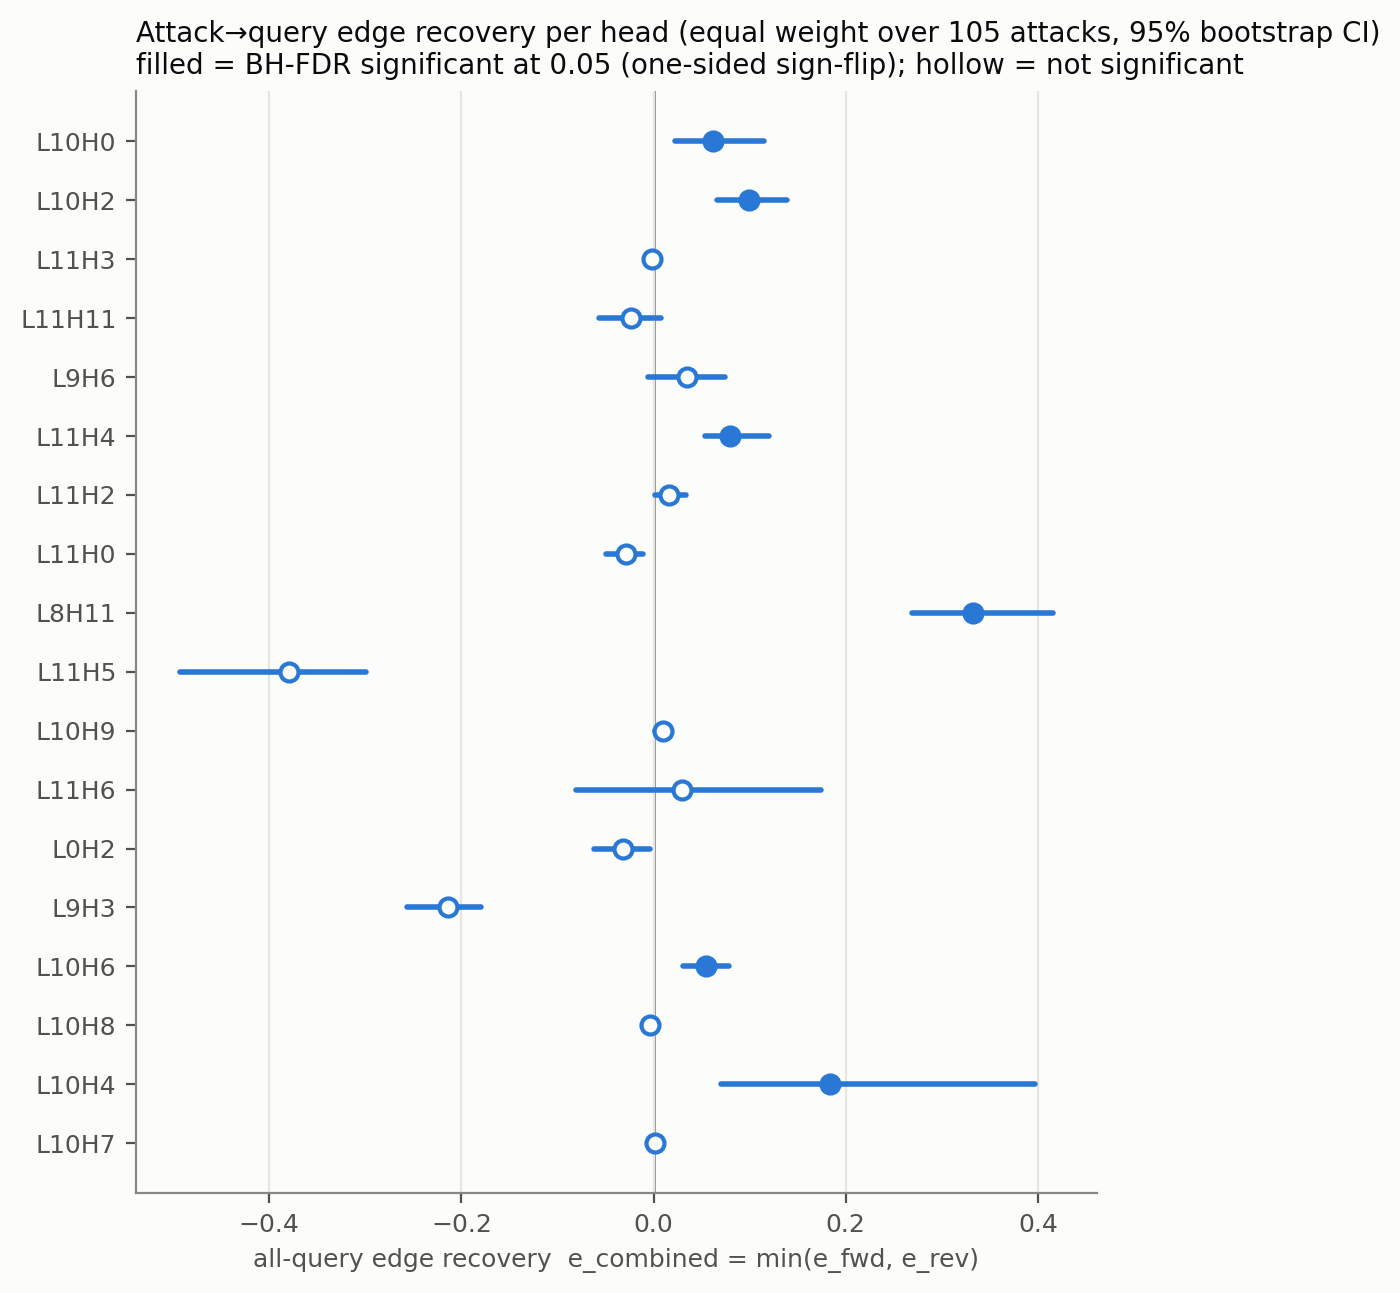
\includegraphics[width=0.72\linewidth]{outputs/plots/fig1_edge_combined_by_head.png}
\caption{All-query \comb{} per head with 95\% bootstrap CIs. Filled markers
are BH-significant.}
\end{figure}

\textbf{Q1: does direct attack$\rightarrow$query flow contribute causally?}
Yes, for part of the effect. Six heads (L8H11, L10H2, L11H4, L10H4, L10H6,
L10H0) are significant at FDR 0.05. For every one of them \fwd{} and \rev{}
agree closely (Fig.~\ref{fig:fwdrev}). Inserting the attacked message into the
control raises the score, and removing it from the attacked run lowers it, by
matching amounts. The pathway therefore passes both sufficiency and necessity
(\textbf{Q3}). This agreement holds for all 18 heads, including the null and
negative ones, which is consistent with a nearly linear response at these
effect sizes.

\textbf{Q2: which heads?} By every summary (Tables~\ref{tab:main},
\ref{tab:robust}), \textbf{L8H11} is the clear leader. The ranking below it
is broadly L10H4, L10H6, L10H2, L10H0 and L11H4. Note that L8H11 was only
9th by whole-head effect in Exp.~11. The heads Exp.~11 ranked highest mostly
do not act through this edge: L11H3 and L11H11 are null, and L10H0 is
modest.

\textbf{Negative edges.} \textbf{L11H5} and \textbf{L9H3} have robustly
negative recovery. For L11H5, 0/105 attacks have a positive raw effect; for
L9H3, 1/105. In these heads the attacked attack$\rightarrow$query message
\emph{opposes} the attack: removing it raises the attacked score further, and
inserting it into the control lowers the score. L11H0, L0H2 and L10H8 are
slightly negative. These are genuine counter-directional routes, not noise.

\begin{figure}[H]\centering
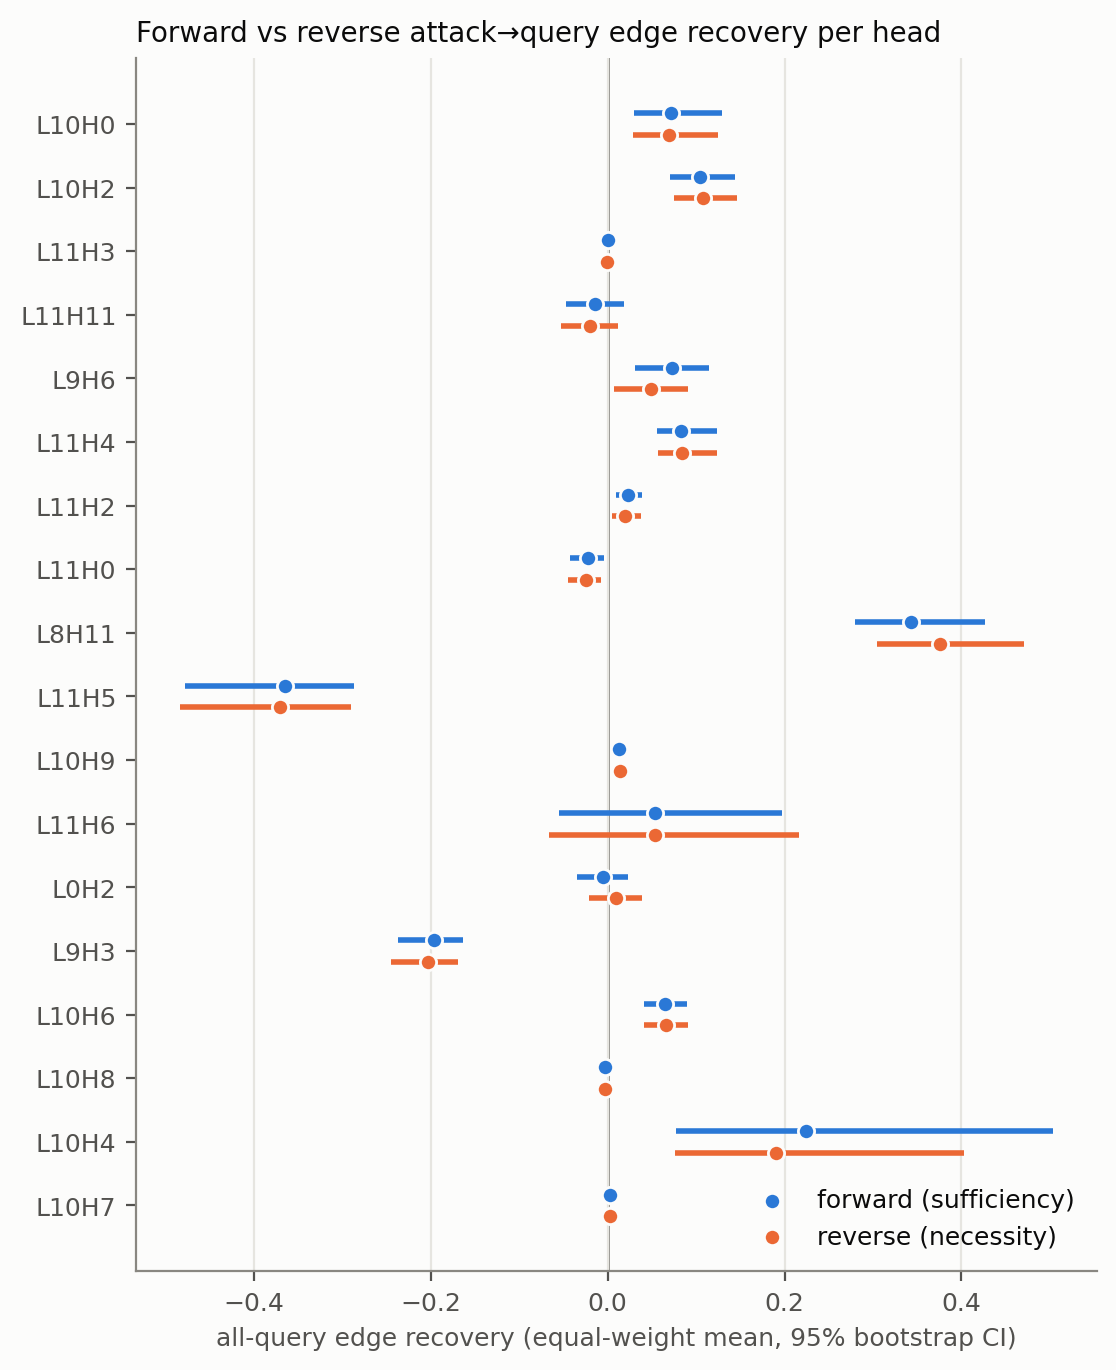
\includegraphics[width=0.72\linewidth]{outputs/plots/fig2_fwd_vs_rev_by_head.png}
\caption{Forward (sufficiency) vs reverse (necessity) all-query recovery.}
\label{fig:fwdrev}
\end{figure}

\subsection{Sensitivity to near-zero attack effects (post-hoc, descriptive)}
\label{sec:robust}
The successful-instance population is dominated by \emph{small} attack
effects: the median $\delta$ is $0.072$ logits, 40\% of examples have
$\delta<0.05$, and 9.5\% have $\delta<0.01$. The per-example ratio $\comb$
therefore explodes for tiny $\delta$. The clearest case: one
\texttt{bar\_start\_2} example has $\delta=2\times10^{-4}$ and a raw effect of
$0.10$--$0.14$ logits, giving $\comb=525$. That single example lifts
L10H4's \texttt{bar\_start\_2} attack mean to $10.7$, which is visible as the
single dark cell in Fig.~\ref{fig:heat}. The pre-registered metric and tests
are left unchanged. Table~\ref{tab:robust} adds descriptive summaries that do
not have this sensitivity; they were added after seeing the results
(DECISIONS.md item 42).

\begin{table}[H]\centering\small
\caption{Post-hoc descriptive robustness (no tests). RoM = per attack
$\min(\overline{\text{raw}_{\text{fwd}}},\overline{\text{raw}_{\text{rev}}})/\bar\delta$,
then an equal-weight mean over attacks. ``$\delta\!\ge\!0.1$'' = headline
mean restricted to examples with $\delta\ge0.1$. ``$>0$'' = fraction of
attacks with a positive raw effect in both directions.}
\label{tab:robust}
\begin{tabular}{lrrrrrr}
\toprule
& \multicolumn{4}{c}{edge (all-query)} & \multicolumn{2}{c}{whole head}\\
\cmidrule(lr){2-5}\cmidrule(lr){6-7}
head & headline \comb & RoM & median & $\delta\!\ge\!0.1$ / $>0$ & RoM & median\\
\midrule
L10H0 & 0.062 & 0.020 & 0.004 & 0.011 / 0.76 & 0.046 & 0.035\\
L10H2 & 0.099 & 0.024 & 0.005 & 0.024 / 0.72 & 0.190 & 0.165\\
L11H3 & $-0.002$ & $-0.001$ & 0.000 & $-0.002$ / 0.63 & 0.079 & 0.052\\
L11H11 & $-0.024$ & $-0.011$ & 0.001 & $-0.009$ / 0.73 & 0.130 & 0.093\\
L9H6 & 0.035 & 0.005 & 0.004 & $-0.002$ / 0.73 & 0.225 & 0.139\\
L11H4 & 0.080 & 0.014 & 0.008 & 0.012 / 0.89 & 0.207 & 0.193\\
L11H2 & 0.016 & 0.006 & 0.001 & 0.006 / 0.83 & 0.073 & 0.044\\
L11H0 & $-0.029$ & $-0.004$ & $-0.005$ & $-0.003$ / 0.21 & $-0.014$ & $-0.026$\\
L8H11 & 0.332 & \textbf{0.085} & \textbf{0.050} & 0.076 / 0.93 & 0.038 & $-0.017$\\
L11H5 & $-0.379$ & $-0.069$ & $-0.050$ & $-0.050$ / 0.00 & $-0.096$ & $-0.088$\\
L10H9 & 0.010 & 0.005 & 0.000 & 0.005 / 0.63 & 0.042 & 0.026\\
L11H6 & 0.030 & $-0.013$ & $-0.025$ & $-0.033$ / 0.27 & 0.118 & 0.084\\
L0H2 & $-0.031$ & 0.011 & $-0.001$ & 0.007 / 0.64 & 0.017 & $-0.009$\\
L9H3 & $-0.214$ & $-0.056$ & $-0.041$ & $-0.054$ / 0.01 & 0.002 & $-0.015$\\
L10H6 & 0.055 & 0.028 & 0.005 & 0.025 / 0.70 & 0.317 & 0.234\\
L10H8 & $-0.004$ & 0.000 & 0.000 & 0.000 / 0.29 & 0.044 & 0.031\\
L10H4 & 0.184 & 0.036 & 0.006 & 0.031 / 0.90 & 0.091 & 0.045\\
L10H7 & 0.001 & 0.001 & 0.000 & 0.001 / 0.57 & 0.027 & 0.009\\
\bottomrule
\end{tabular}
\end{table}

For every head, the robust summaries agree with the headline in
\emph{sign}, and the ranking of the six significant heads is essentially
preserved. The \emph{magnitudes} are 3--5$\times$ smaller: L8H11 accounts
for roughly 5--8\% of the attack effect, and the other significant heads
1--4\%. L10H4's headline value of 0.18 is mostly the one-example outlier
above; its robust effect (0.03--0.04) is still positive on 90\% of attacks.
L11H6's headline 0.030 turns negative under the robust summaries, so it
should be read as null to slightly negative. The one qualitative change
concerns L0H2: its negative headline and CI turn slightly positive under RoM
and $\delta\ge0.1$, so it is best read as null.

\subsection{Edge vs whole head (secondary)}
\begin{figure}[H]\centering
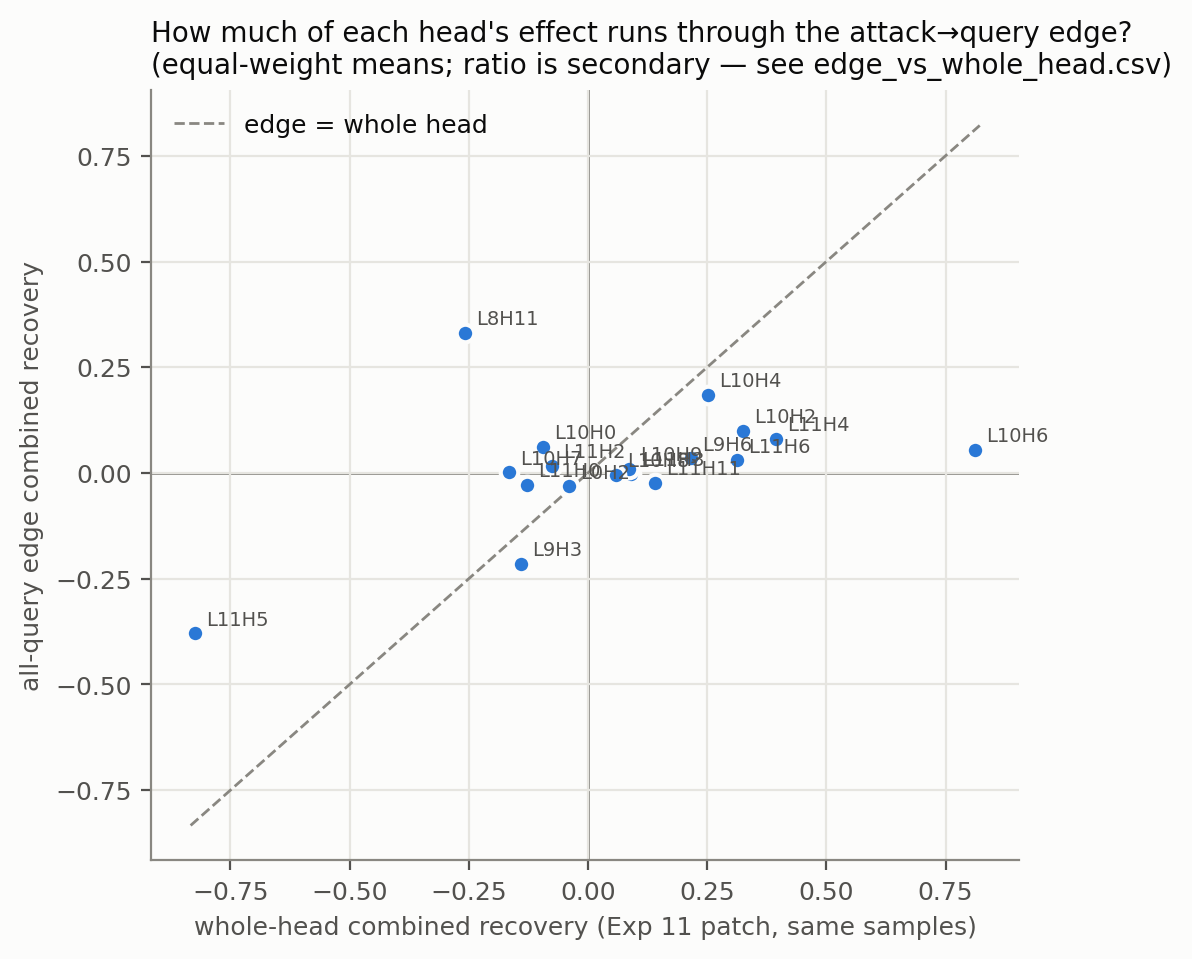
\includegraphics[width=0.6\linewidth]{outputs/plots/fig3_edge_vs_whole_head.png}
\caption{Equal-weight edge \comb{} vs whole-head \comb{} (same samples and
baselines). Dashed: edge = whole head.}
\end{figure}

\textbf{Q4: how much of each head's effect goes through the direct edge?}
Mostly a small part. Under the robust RoM view:
\begin{itemize}[nosep]
\item \textbf{Most heads:} the whole-head effect is much larger than the
  edge effect, for example L10H6 (0.317 vs 0.028), L9H6 (0.225 vs 0.005),
  L11H4 (0.207 vs 0.014) and L10H2 (0.190 vs 0.024). These heads mainly
  matter through other routes: messages into document or template
  positions, attack information arriving indirectly, or the non-attack part
  of their output at query positions.
\item \textbf{Several heads important in Exp.~11} (L11H3, L11H11, L9H6)
  have essentially \emph{no} direct-edge effect.
\item \textbf{L8H11 is the exception.} Its edge effect (0.085) exceeds its
  whole-head effect (0.038 RoM; negative median and negative equal-weight
  mean). The direct attack$\rightarrow$query message pushes the score up,
  while the rest of the head's output pushes the other way.
\end{itemize}
Ratios are listed in \texttt{edge\_vs\_whole\_head.csv}. They are unstable
wherever the whole-head denominator is small or negative (e.g.\ L9H3,
L8H11), so we do not interpret them individually.

\subsection{Consistency across the 105-attack sweep}
\begin{figure}[H]\centering
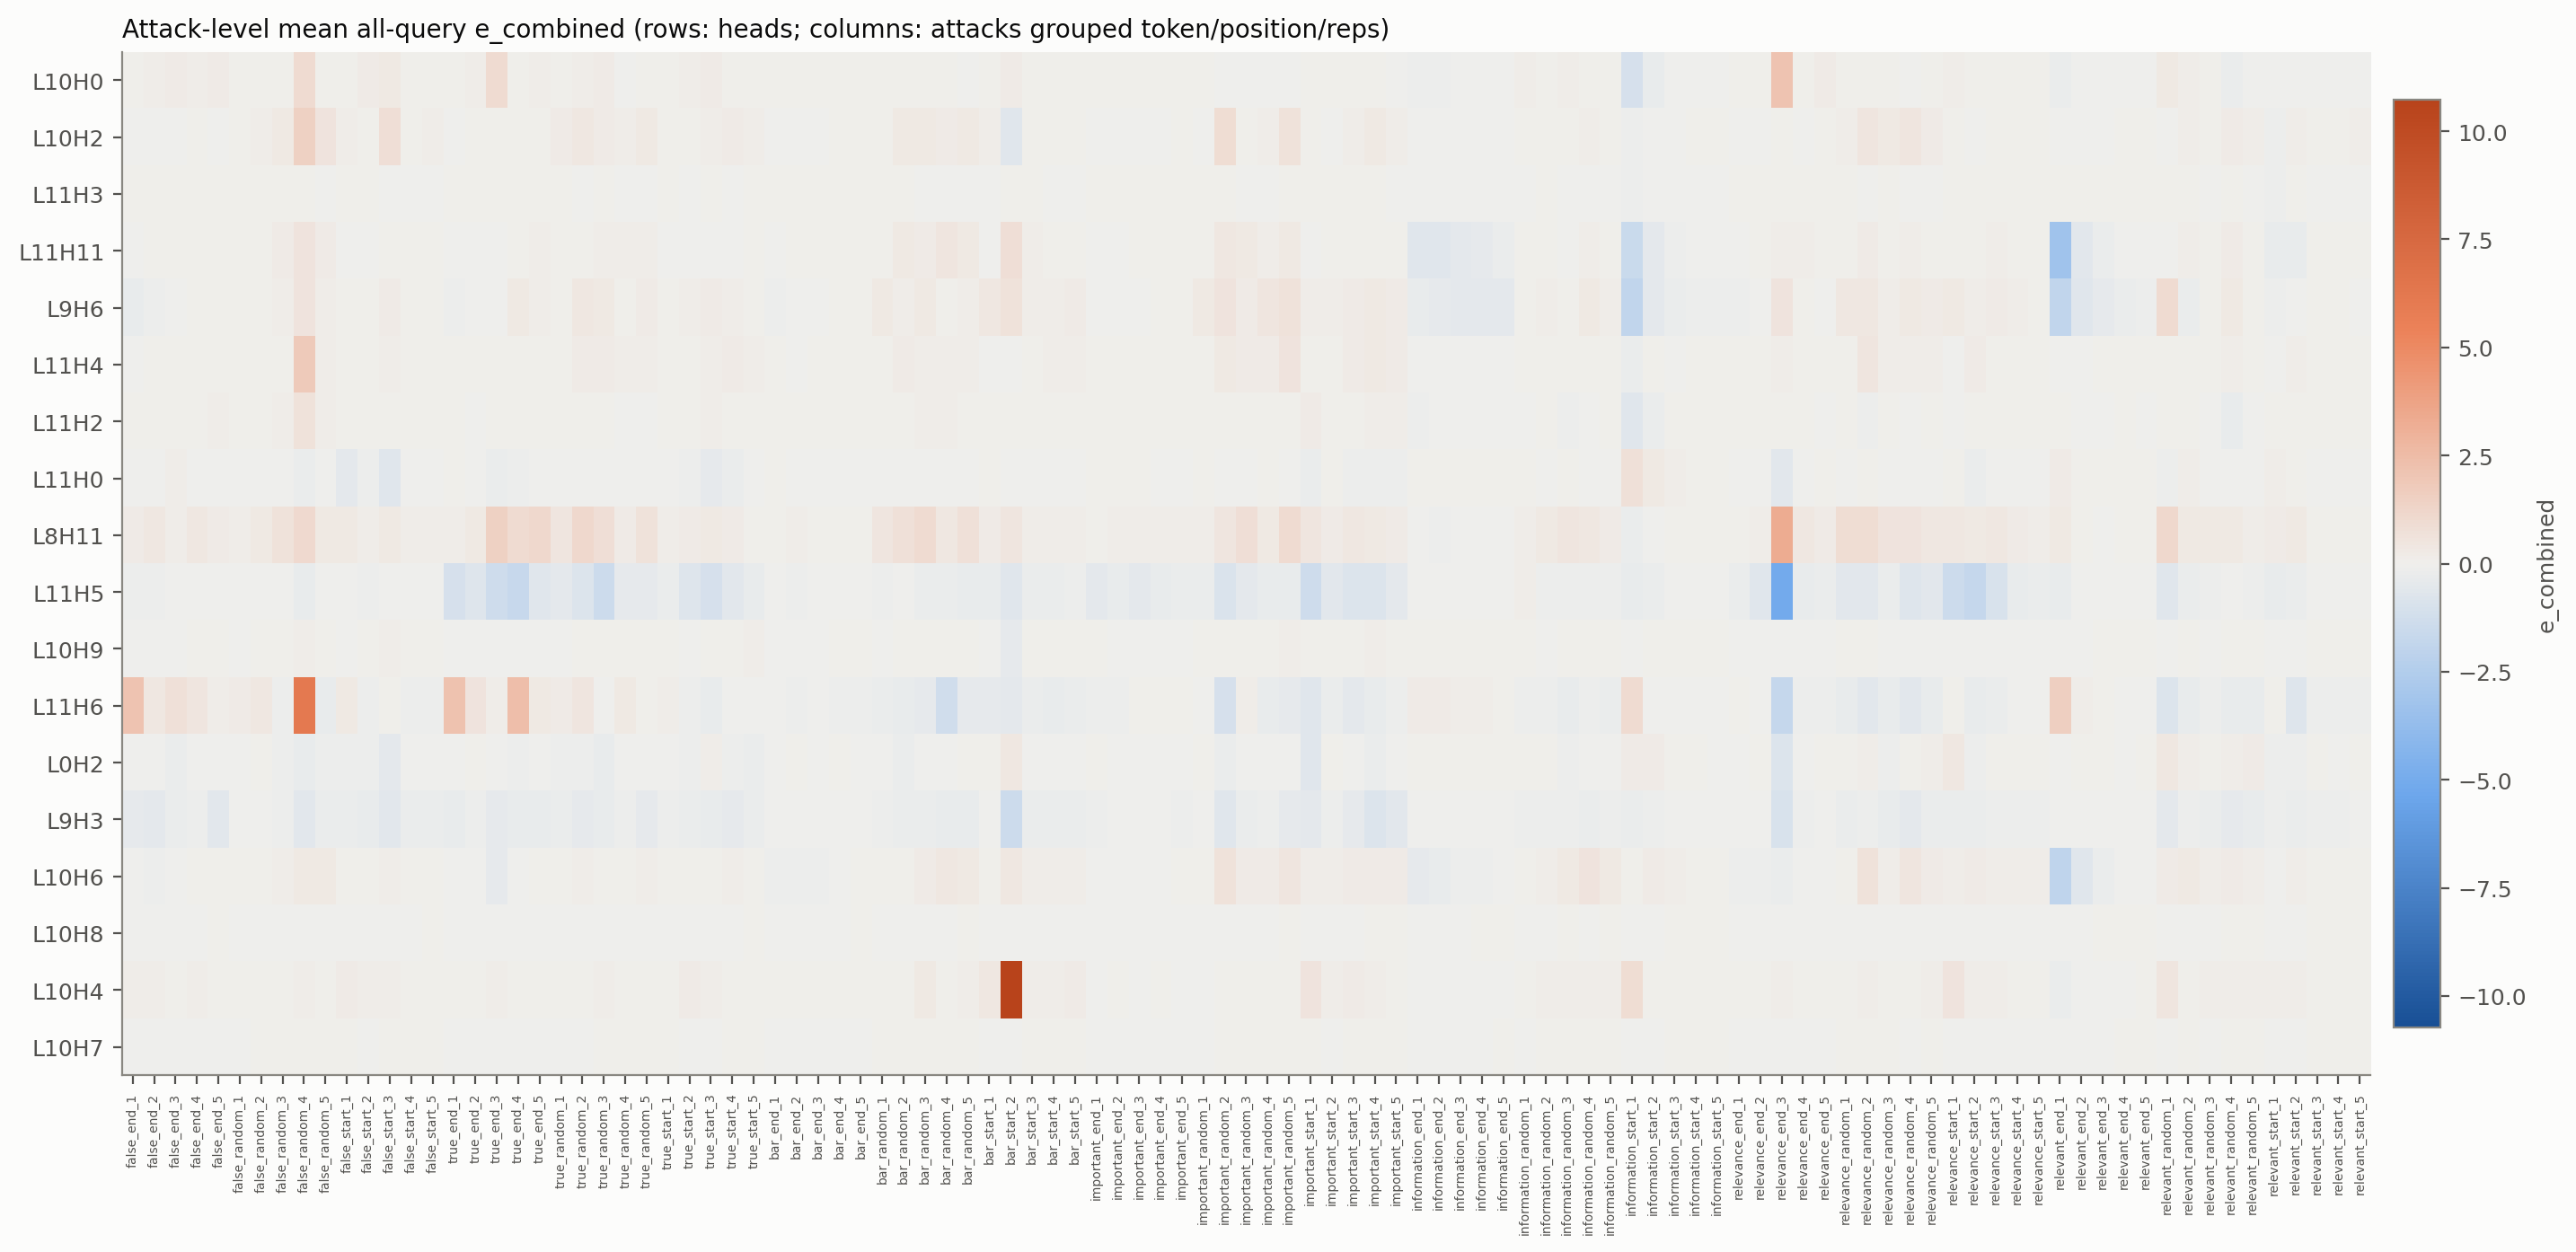
\includegraphics[width=\linewidth]{outputs/plots/fig5_attack_head_heatmap.png}
\caption{Attack-level mean \comb{} (heads $\times$ attacks). The single
saturated cell (L10H4, \texttt{bar\_start\_2}) is the $\delta=2\times10^{-4}$
example discussed in \S\ref{sec:robust}.}
\label{fig:heat}
\end{figure}
\begin{figure}[H]\centering
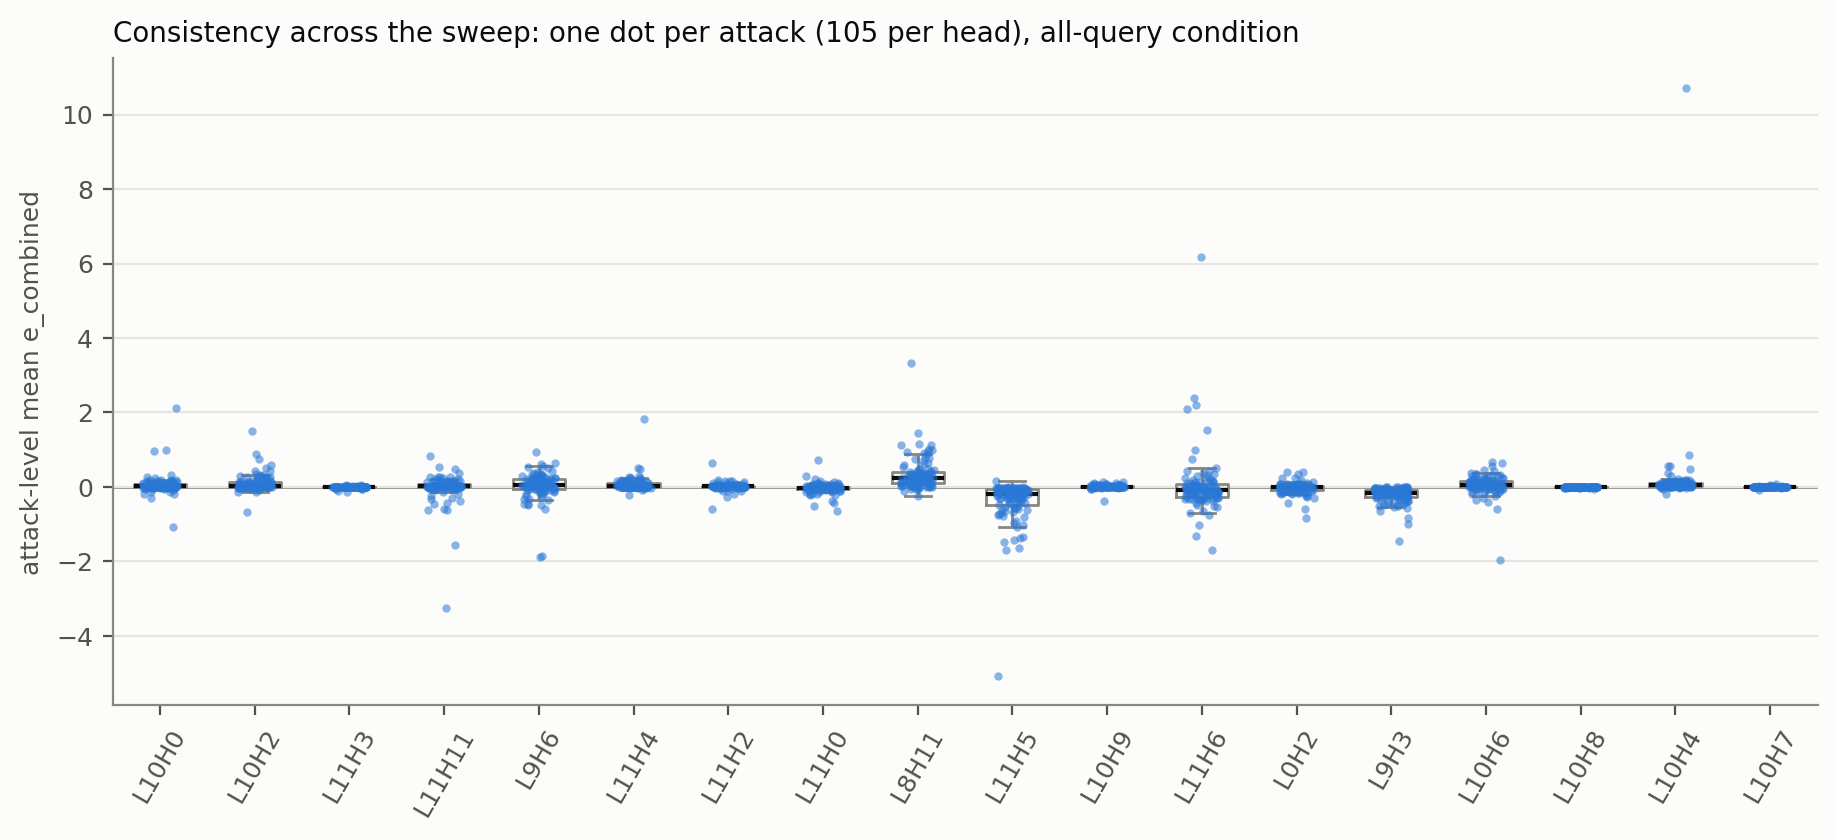
\includegraphics[width=0.8\linewidth]{outputs/plots/fig4_attack_level_distribution.png}
\caption{Distribution of the 105 attack-level means per head.}
\end{figure}

\textbf{Q6: are the effects consistent across attacks?}
\begin{itemize}[nosep]
\item \textbf{Consistent signs.} Raw effects are positive in both directions
  on 93\% of attacks for L8H11, 90\% for L10H4, 89\% for L11H4, and
  70--76\% for L10H0, L10H2 and L10H6. They are negative on all 105
  attacks for L11H5 and on 104/105 for L9H3.
\item \textbf{L8H11 by attack.} Largest for \texttt{relevance} and
  \texttt{true} tokens (attack-level means 0.59 and 0.54) and smallest for
  \texttt{information} (0.06). By position: random 0.53, end 0.29,
  start 0.18.
\item \textbf{L10H2.} Almost entirely driven by random-position attacks
  (0.24, vs 0.06 start and 0.00 end).
\item \textbf{L11H5.} Opposes the attack most strongly for \texttt{relevance}
  ($-0.90$) and \texttt{true} ($-0.77$).
\item \textbf{Outliers.} Individual attack means range widely, e.g.\ L11H6
  from $-1.7$ to $6.2$. These extremes trace back to tiny-$\delta$ examples.
\end{itemize}

\subsection{Individual query tokens (descriptive)}
\begin{figure}[H]\centering
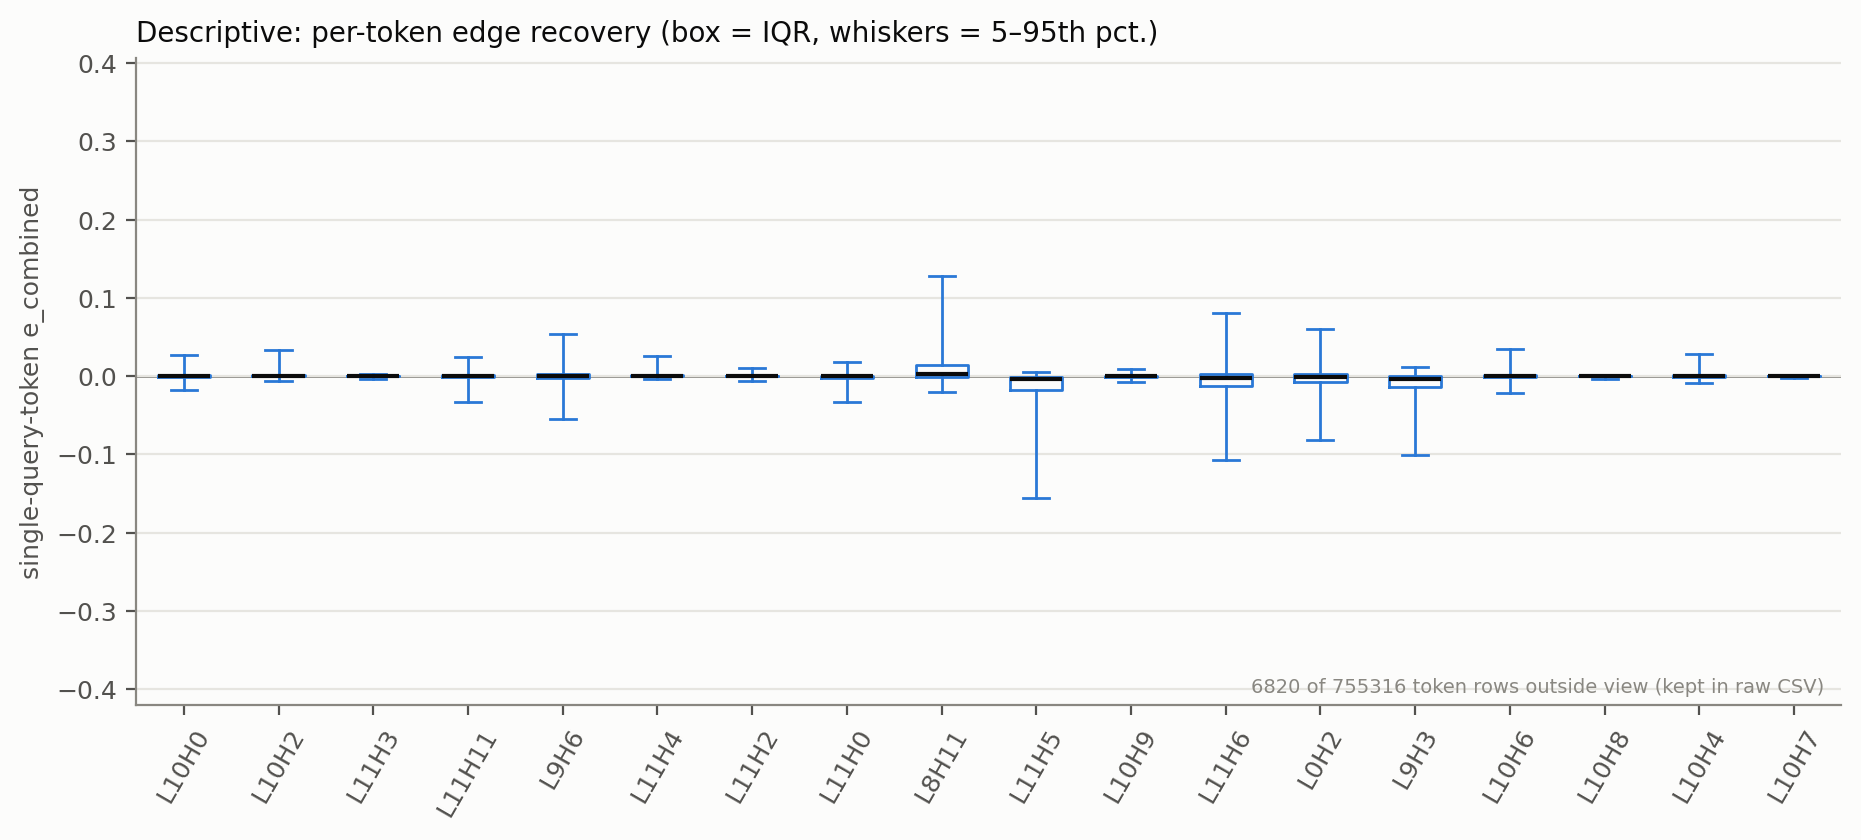
\includegraphics[width=0.8\linewidth]{outputs/plots/fig6_token_distribution.png}
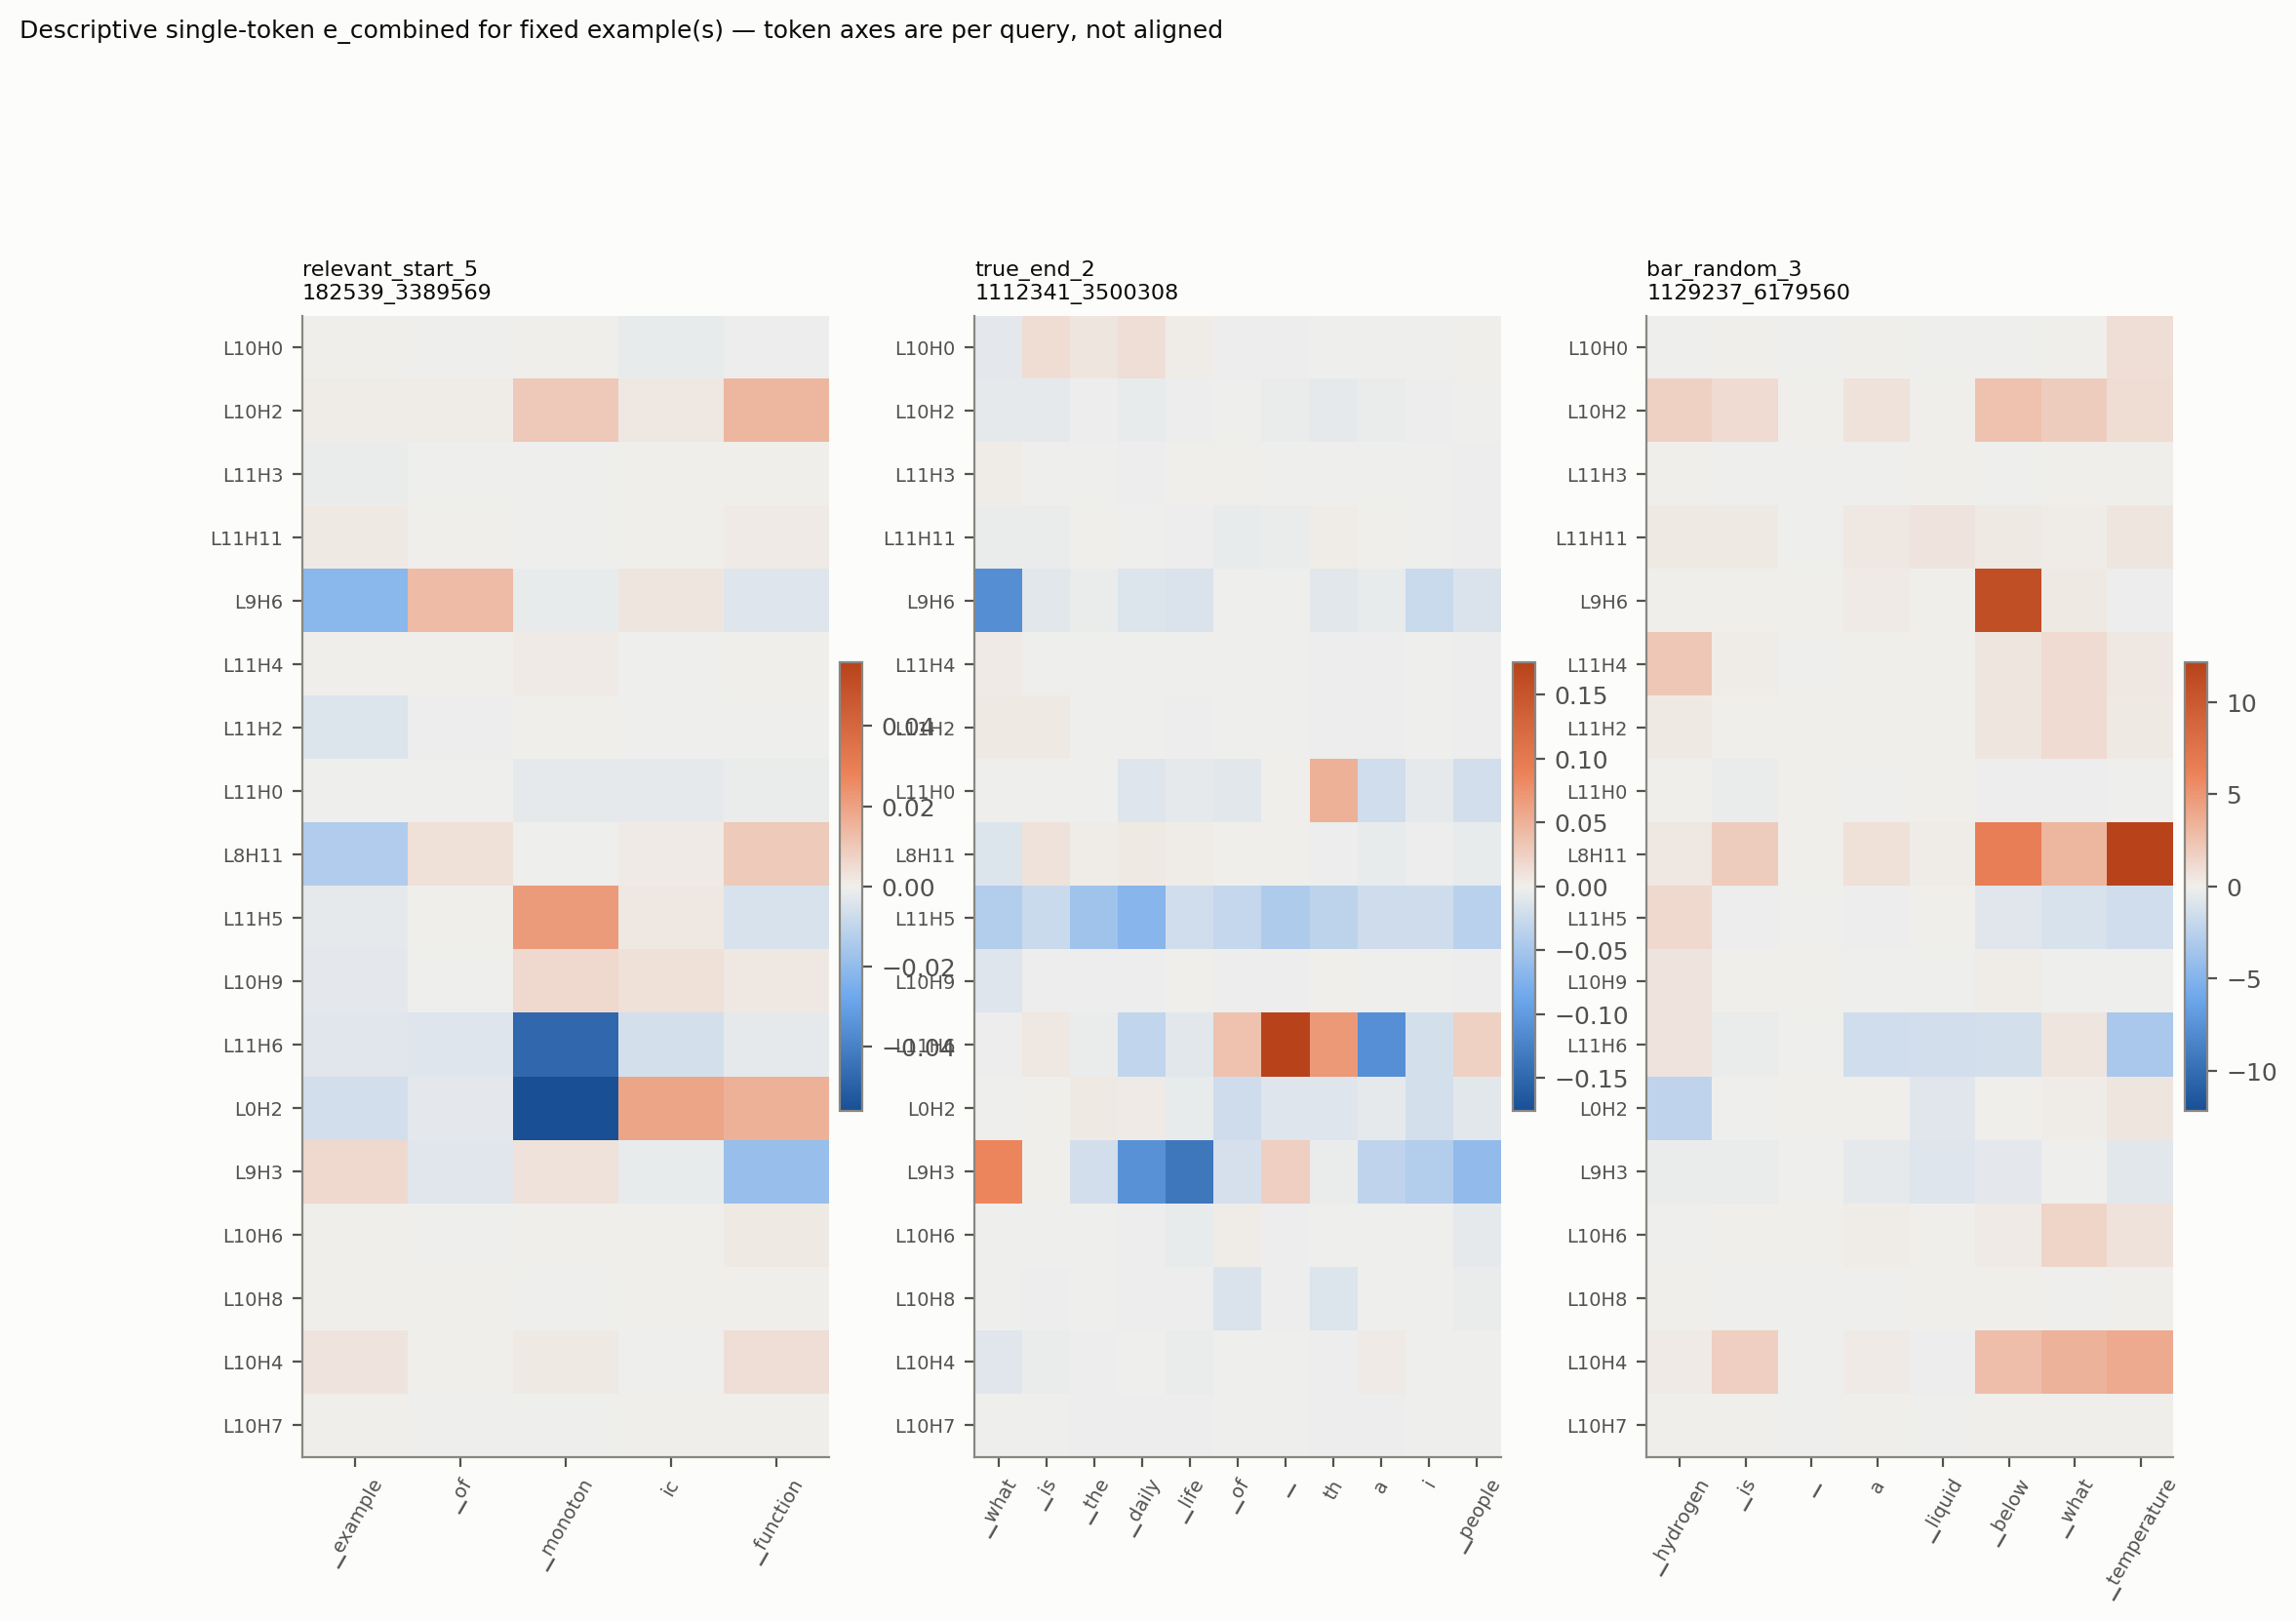
\includegraphics[width=\linewidth]{outputs/plots/fig7_token_examples.png}
\caption{Top: per-token \comb{} distributions. Bottom: heads $\times$ query
tokens for fixed examples (token axes are per query, not aligned across
queries).}
\end{figure}

\textbf{Q5: what do single-token interventions show?}
\begin{itemize}[nosep]
\item \textbf{Small, diffuse per-token effects.} Median per-token \comb{} is
  about 0 for most heads (L8H11: 0.002). The fraction of positive tokens is
  highest for L8H11 (69\%) and L11H4 (63\%) and lowest for L11H5 (14\%).
\item \textbf{No clear location.} The top-recovery token is neither
  systematically first nor last in the query (typically 10--25\% and
  13--25\% of examples, respectively). L11H4 is the exception: its top token
  is the first query token in 40\% of examples.
\item \textbf{Frequent top tokens for L8H11.} These are
  \texttt{\_definition} (615 of 5{,}250 examples), \texttt{\_the},
  \texttt{\_is}, \texttt{\_of}, \texttt{\_description} and
  \texttt{\_define}. This partly reflects how often these words occur in
  MS~MARCO queries; no alignment across queries is implied.
\item \textbf{Near-additivity.} The sum of single-token raw effects matches
  the explicit all-query raw effect to within $5\times10^{-4}$ logits (equal-weight means) for
  every head (\texttt{token\_summary\_by\_head.csv}). Each all-query value
  was measured by its own explicit intervention, so this is an empirical
  finding and says nothing beyond this small-effect regime.
\end{itemize}

\section{Interpretation and limits}
\begin{itemize}[nosep]
\item \textbf{Main result.} Direct attack$\rightarrow$query communication
  through L8H11, and more weakly through L10H0/2/4/6 and L11H4, causally
  mediates a small but consistent part of the attack. It passes both the
  sufficiency and the necessity test. L11H5 and L9H3 carry opposing direct
  messages.
\item \textbf{Mostly not direct.} This direct edge explains only a few
  percent of each head's effect, except for L8H11. Most of the 18 heads'
  causal importance, and most of the query-representation change seen in
  Exp.~6/12, must arise through other routes: attack$\rightarrow$document
  or attack$\rightarrow$template messages, multi-hop relays, or downstream
  mixing.
\item \textbf{What this does not show:}
  \begin{itemize}[nosep]
  \item that this is the only route;
  \item that the heads' effects add up (heads were tested one at a time);
  \item that attention mass explains importance: L8H11's mean attention
    mass on $A$ from query positions is only 0.015, lower than several null
    heads (e.g.\ L11H6 0.027, L9H3 0.024);
  \item that token effects are linear outside this regime.
  \end{itemize}
\item \textbf{The headline metric.} It is dominated by near-zero-$\delta$
  examples. Future experiments on this population should pre-register a
  pooled (ratio-of-means) or $\delta$-thresholded summary alongside it.
\end{itemize}

\section*{Reproducibility}
Code, configurations, the immutable manifest (sha256 \texttt{686db9cb\ldots})
and all raw per-example outputs are in
\texttt{patch\_code/analysis/15\_monot5\_attack\_to\_query\_flow/}. The full
run was SLURM job 1420506 (1$\times$L40, about 50 minutes of compute including one SLURM requeue that resumed from per-attack checkpoints). See README.md
and DECISIONS.md.

\end{document}
